\documentclass[aspectratio=169,10pt]{beamer}
\usetheme{Madrid}
\usepackage{tikz}
\usepackage{pgfplots}
\usetikzlibrary{positioning}
\pgfplotsset{compat=1.18}
\title{Monty Hall: Probability After a Reveal}
\subtitle{Week 10 — a sample space, a host rule, and simulations}
\author{COMSC 2043 • Discrete Structures and Critical Thinking}
\date{October 21, 2026}
\begin{document}
\frame{\titlepage}
\begin{frame}{State the rules before calculating}
\begin{itemize}\item Three doors; one car, two goats.\item You choose door 1.\item The host knows the car location, opens an unchosen goat door, and chooses uniformly if both doors are goats.\item You may stay with door 1 or switch to the remaining closed door.\end{itemize}

\note{Point from the chosen door to the host action and remaining alternative. Keep the host's information and constraint explicit.}\par\end{frame}
\begin{frame}{The nine equally likely cases}
Each ordered pair (your pick, car location) has probability $1/9$.\medskip
\centering\begin{tabular}{c|ccc} & Car 1 & Car 2 & Car 3\\\hline Pick 1 & H opens 2 or 3 & H opens 3 & H opens 2\\Pick 2 & H opens 3 & H opens 1 or 3 & H opens 1\\Pick 3 & H opens 2 & H opens 1 & H opens 1 or 2\end{tabular}
\medskip\raggedright By symmetry, the three rows have identical stay/switch outcomes.\note{Walk through the displayed information in order. Ask students for a prediction before stating the conclusion.}\end{frame}
\begin{frame}{The three symmetric cases}
Assume your pick is door 1.\\[2mm]\begin{tabular}{c|c|c}Car location&Host opens&Switch outcome\\\hline1&2 or 3 (equally)&Lose\\2&3&Win\\3&2&Win\end{tabular}\\[3mm]Stay wins in one of the three cases; switching wins in two.\note{Walk through the displayed information in order. Ask students for a prediction before stating the conclusion.}\end{frame}
\begin{frame}{Conditional probability is a ratio inside an event}
For events $A,B$ with $P(B)>0$, definition: $P(A\mid B)=P(A\cap B)/P(B)$.\\[3mm]After a host reveal, the relevant sample space is the set of cases compatible with that reveal and the host's rule.\\[2mm]The denominator changes when we condition.\note{Walk through the displayed information in order. Ask students for a prediction before stating the conclusion.}\end{frame}
\begin{frame}{Bayes: host opens door 3}
Let $C_i$ mean car behind door $i$; let $O_3$ mean host opens door 3.\\[2mm]$P(C_1)=P(C_2)=P(C_3)=1/3$.\\$P(O_3\mid C_1)=1/2$, $P(O_3\mid C_2)=1$, $P(O_3\mid C_3)=0$.\\[2mm]$P(O_3)=\sum_i P(O_3\mid C_i)P(C_i)=1/6+1/3=1/2$.\\[2mm]$P(C_1\mid O_3)=((1/2)(1/3))/(1/2)=1/3$; hence $P(C_2\mid O_3)=2/3$. Switch.\note{Walk through the displayed information in order. Ask students for a prediction before stating the conclusion.}\end{frame}
\begin{frame}{Bayes denominator: add the paths that show door 3}
Let $O_3$ mean the host opens door 3. The probability paths are: $C_1$ contributes $(1/3)(1/2)=1/6$; $C_2$ contributes $(1/3)(1)=1/3$; $C_3$ contributes $(1/3)(0)=0$. Thus
\[P(O_3)=1/6+1/3+0=1/2.\]
\centering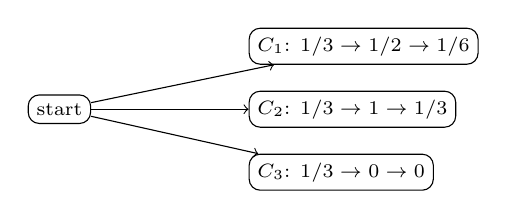
\begin{tikzpicture}[node distance=9mm,every node/.style={draw,rounded corners,inner sep=3pt,font=\scriptsize}]
\node (s) {start};\node[right=20mm of s,yshift=8mm] (a) {$C_1$: $1/3\to1/2\to1/6$};\node[right=20mm of s] (b) {$C_2$: $1/3\to1\to1/3$};\node[right=20mm of s,yshift=-8mm] (c) {$C_3$: $1/3\to0\to0$};\draw[->](s)--(a);\draw[->](s)--(b);\draw[->](s)--(c);\end{tikzpicture}
\note{Add only the joint probabilities of paths where the host opens door 3. These terms form Bayes' denominator.}
\end{frame}
\begin{frame}{$n$ doors: one closed alternative}
You pick one of $n$ doors. The first pick is correct with probability $1/n$.\\A knowing host opens $n-2$ goats, leaving one alternative.\\Switch wins exactly when the first pick was wrong: $P(\text{switch wins})=(n-1)/n$.\\For $n=100$, this is $99/100$.\note{Walk through the displayed information in order. Ask students for a prediction before stating the conclusion.}\end{frame}
\begin{frame}{Open $k$ goats; switch to one chosen survivor}
\textbf{Claim:} With a uniform choice among survivors, each gets an equal share.
\begin{align*}
P(\text{first pick wrong})&=(n-1)/n &&\text{there are $n-1$ wrong doors}\pause\\
\text{alternatives left}&=n-1-k &&\text{the host opens $k$ goats}\pause\\
P(\text{win on specified door})&=\frac{(n-1)/n}{n-1-k} &&\text{split wrong-pick chance evenly}\pause\\
&=\frac{n-1}{n(n-1-k)} &&\text{simplify}\pause\\
(n,k)=(5,2)&\Rightarrow P=4/10 &&\text{each of two doors gets $0.4$}
\end{align*}
\end{frame}
\begin{frame}{Monty Fall: a random host}
\textbf{Claim:} Given a goat is shown, staying and switching are equally likely to win.
\begin{align*}
P(C=1)&=P(C=2)=P(C=3)=1/3 &&\text{car is equally likely}\pause\\
P(G\mid C=1)&=1,\quad P(G\mid C=2)=P(G\mid C=3)=1/2 &&\text{random host avoids car}\pause\\
P(G)&=1/3+(1/3)(1/2)+(1/3)(1/2)=2/3 &&\text{add goat-showing branches}\pause\\
P(C=1\mid G)&=(1/3)/(2/3)=1/2 &&\text{stay wins only when car is picked}\pause\\
P(C\ne1\mid G)&=((1/3)(1/2)+(1/3)(1/2))/(2/3)=1/2 &&\text{switch wins on other branches}
\end{align*}
\centering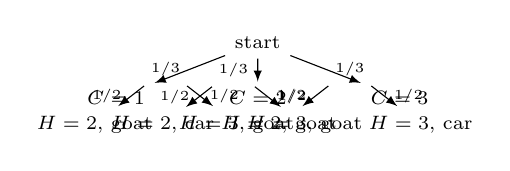
\begin{tikzpicture}[level distance=7mm,sibling distance=18mm,every node/.style={font=\scriptsize},edge from parent/.style={draw,-latex}]
\node {start}
 child {node {$C=1$} edge from parent node[left,font=\tiny] {$1/3$}
   child {node {$H=2$, goat} edge from parent node[left,font=\tiny] {$1/2$}}
   child {node {$H=3$, goat} edge from parent node[right,font=\tiny] {$1/2$}}}
 child {node {$C=2$} edge from parent node[left,font=\tiny] {$1/3$}
   child {node {$H=2$, car} edge from parent node[left,font=\tiny] {$1/2$}}
   child {node {$H=3$, goat} edge from parent node[right,font=\tiny] {$1/2$}}}
 child {node {$C=3$} edge from parent node[right,font=\tiny] {$1/3$}
   child {node {$H=2$, goat} edge from parent node[left,font=\tiny] {$1/2$}}
   child {node {$H=3$, car} edge from parent node[right,font=\tiny] {$1/2$}}};
\end{tikzpicture}
\end{frame}
\begin{frame}{Monty Crawl: a leftmost-door rule}
\textbf{Claim:} Switching wins with probability $2/3$ before the reveal.
\begin{align*}
P(C=1)&=P(C=2)=P(C=3)=1/3 &&\text{three equally likely locations}\pause\\
C=1&\Rightarrow H=2,\;\text{switch loses} &&\text{first pick has the car}\pause\\
C=2&\Rightarrow H=3,\;\text{switch wins} &&\text{host opens leftmost eligible door}\pause\\
C=3&\Rightarrow H=2,\;\text{switch wins} &&\text{host opens the remaining goat}\pause\\
P(\text{switch wins})&=0+1/3+1/3=2/3 &&\text{add winning cases}
\end{align*}
\end{frame}
\begin{frame}{Three Prisoners}
\textbf{Claim:} Hearing that B is not pardoned leaves A at $1/3$ and C at $2/3$.
\centering\small
\begin{tabular}{c|c|c|c}\text{pardoned}&P(\text{case})&P(\text{guard says B})&P(\text{joint})\\\hline A&1/3&1/2&1/6\\B&1/3&0&0\\C&1/3&1&1/3\end{tabular}
\begin{align*}
P(\text{guard says B})&=1/6+0+1/3=1/2 &&\text{add the B-name paths}\pause\\
P(A\mid\text{guard says B})&=(1/6)/(1/2)=1/3 &&\text{A's chance is unchanged}\pause\\
P(C\mid\text{guard says B})&=(1/3)/(1/2)=2/3 &&\text{the remaining chance is C}
\end{align*}
\end{frame}
\begin{frame}{Simulation checks a model's long-run rate}
The simulator repeats the stated random experiment. For $N$ independent trials, the law of large numbers says the observed fraction tends toward the model probability as $N$ grows.\\[2mm]It does not prove the assumptions or promise a close result for a small $N$. Seeded measurement (10,000 games): stay $3412/10000=0.3412$; switch $6588/10000=0.6588$.\\
\centering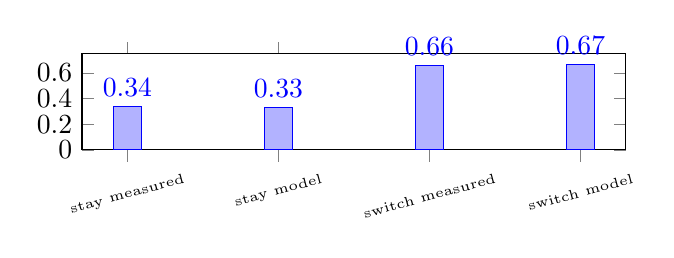
\begin{tikzpicture}\begin{axis}[ybar,width=.7\linewidth,height=2.8cm,ymin=0,ymax=.75,symbolic x coords={stay measured,stay model,switch measured,switch model},xtick=data,xticklabel style={font=\tiny,rotate=15},nodes near coords]\addplot coordinates {(stay measured,.3412) (stay model,.3333) (switch measured,.6588) (switch model,.6667)};\end{axis}\end{tikzpicture}\note{Walk through the displayed information in order. Ask students for a prediction before stating the conclusion.}\end{frame}
\begin{frame}{Playground: Buffon's hot dogs}
\textbf{Claim:} The crossing rate estimates $\pi$ when segment length equals line spacing.
\begin{align*}
P(\text{cross}\mid\theta)&=(\ell/t)\sin\theta &&\text{center must be near a line}\pause\\
p&=\frac1\pi\int_0^\pi(\ell/t)\sin\theta\,d\theta &&\text{average over orientations}\pause\\
&=2\ell/(\pi t) &&\text{evaluate the integral}\pause\\
\widehat p&=\text{crossings}/N &&\text{measure the fraction}\pause\\
\widehat\pi&=2\ell/(t\widehat p) &&\text{solve for $\pi$}
\end{align*}
\end{frame}
\begin{frame}{Playground: darts and birthdays}
\textbf{Claim:} Area and complementary counting give exact model probabilities.
\begin{align*}
P(\text{dart hits})&=\pi/4 &&\text{quarter-circle area over square area}\pause\\
\widehat\pi&=4(\text{hits}/N) &&\text{rearrange the measured rate}\pause\\
P(\text{no birthday match})&=\prod_{i=0}^{n-1}(365-i)/365 &&\text{multiply no-match chances}\pause\\
P(\text{a match})&=1-\prod_{i=0}^{n-1}(365-i)/365 &&\text{take the complement}\pause\\
P(\text{match at }n=23)&\approx0.5073 &&\text{more than one half}
\end{align*}
\end{frame}
\begin{frame}{Playground: collecting every coupon}
\textbf{Claim:} Collecting $n$ equally likely types takes $nH_n$ draws on average.
\begin{align*}
P(\text{new type}\mid k\text{ held})&=(n-k)/n &&\text{$n-k$ unseen types}\pause\\
E(W_k)&=n/(n-k) &&\text{geometric wait is reciprocal}\pause\\
E(T)&=\sum_{k=0}^{n-1}n/(n-k) &&\text{add stage waits}\pause\\
&=n\sum_{j=1}^n1/j=nH_n &&\text{rewrite as harmonic sum}\pause\\
E(T)_{n=10}&\approx29.29 &&\text{compare with simulated mean}
\end{align*}
\end{frame}
\begin{frame}{Secretary rule: derive the finite-$n$ chance}
Set $r=\lfloor n/e\rfloor$. Skip the first $r$ applicants and remember their best. If the overall best is at position $j>r$, the rule selects it exactly when the best of the first $j-1$ positions lies among the first $r$.\\That probability is $r/(j-1)$, while the overall best is at $j$ with probability $1/n$. Therefore
\[P(\text{success})=\sum_{j=r+1}^{n}\frac{r}{n(j-1)}\longrightarrow 1/e.\]
For $n=100$, $r=36$ and the finite sum is approximately $0.3710$ (the limit is $1/e\approx0.3679$).
\note{Condition on the position j of the best applicant. Explain why the rule wins only when the best among the first j−1 is in the skipped group. The playground compares the finite sum with simulation.}
\end{frame}
\begin{frame}{What to remember}
\begin{itemize}\item A probability answer depends on the sample space and the host's rule.\item A reveal can change conditional probabilities; it does not erase the original choice.\item Derive the model first, then use simulation to check its numerical behavior.\end{itemize}\note{Walk through the displayed information in order. Ask students for a prediction before stating the conclusion.}\end{frame}
\end{document}
